\documentclass[12pt, a4paper]{article}
\usepackage[utf8]{inputenc}
\usepackage[russian]{babel}
\usepackage[pdftex]{graphicx, color}
\usepackage{amsmath, amsfonts, amssymb, amsthm}
\usepackage[left=2cm,right=2cm,top=1.5cm,bottom=2cm]{geometry}
\usepackage{indentfirst}

\usepackage{setspace}
\onehalfspacing
\graphicspath{{pics/}}

\begin{document}

    \thispagestyle{empty}

    \begin{singlespace}
    \begin{titlepage}
        \begin{center}
            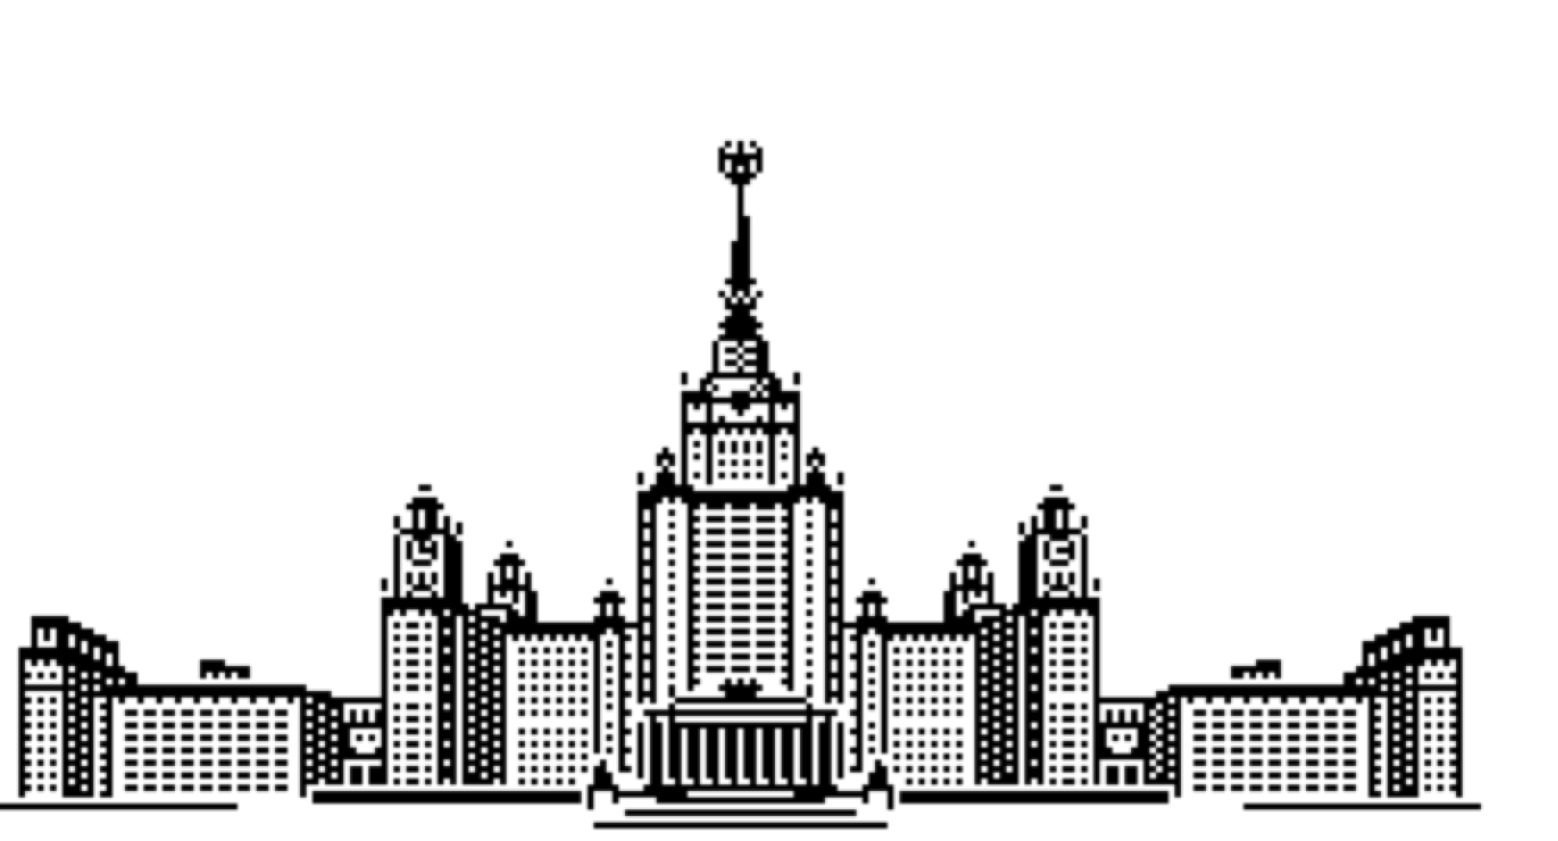
\includegraphics[height = 3cm]{msu.png}

            {\scshape Московский государственный университет имени М.~В.~Ломоносова}\\
            Факультет вычислительной математики и кибернетики\\
            Кафедра математических методов прогнозирования\\
            \centerline{\hfill\hrulefill\hrulefill\hrulefill\hrulefill\hfill}

            \vfill

            {\LARGE Отчет к третьему практическому заданию по МОМО: \\ Выпуклая негладкая, условная и структурная оптимизация}

            \vspace{1cm}

        \end{center}

        \vfill

        \begin{flushright}
            Студент 517 группы:\\
                \textit{Оспанов А.М.}

            \vspace{5mm}

        \end{flushright}

        \vfill

        \begin{center}
            Москва, 2016
        \end{center}
    \end{titlepage}
    \end{singlespace}

    \newpage


    \section{Введение}
    В данной работе будут выведены вспомогательная функция и ньютоновское направление для метода барьеров, будет реализован модуль l1linreg.py
    с реализацией проксимального метода, субградиентного метода и метода барьеров.

    Код написан на языке Python 3 с использованием библиотеки numpy.


    \section{$\phi_\tau(w^+, w^-)$ и вывод $(p_k^+, p_k^-)$}

    Рассмотрим задачу оптимизации следующего вида:

    $$
    \begin{cases}
        f(x) \to min, & x \in \mathbb{D} \subseteq \mathbb{R}^n\\
        g_i(x) \leq 0, & i = 1, ..., m\\
    \end{cases}
    $$

    Тогда вспомогательная фунцкия для метода барьеров будет иметь следующий вид:

    $$\phi_\tau(x) = \tau f(x) - \displaystyle\sum_{i=1}^{m}log(-g_i(x))$$

    Учитывая общий вид, напишем вспомогательную ф-ю для задачи (5):

    $\phi_\tau(w^+, w^-) = \dfrac{\tau}{2n}||X(w^+ - w^-) - y||_2^2 + \tau\lambda\vec{1}(w^+ + w^-) - \displaystyle\sum_{i=1}^{m}(log(w_i^+) + log(w_i^-))$

    \medskip

    Далее, чтобы выписать систему линейных уравнений, задающую ньютоновоское направление $(p_k^+, p_k^-)$, нужно посчитать градиенты и гессианы:

    $\nabla_{w^+} \phi_\tau = \dfrac{\tau}{n} X^T(X(w^+ - w^-) - y) + \tau\lambda\vec{1} - \widetilde{w}^+$, где $\widetilde{w}^+ = \Big(\dfrac{1}{w_1^+}, ..., \dfrac{1}{w_d^+}\Big)$

    $\nabla_{w^-} \phi_\tau = -\dfrac{\tau}{n} X^T(X(w^+ - w^-) - y) + \tau\lambda\vec{1} - \widetilde{w}^-$, где $\widetilde{w}^- = \Big(\dfrac{1}{w_1^-}, ..., \dfrac{1}{w_d^-}\Big)$

    $\nabla_{w^+}^2 \phi_\tau = \dfrac{\tau}{n} X^TX + diag(\widetilde{w}_s^+)$, где $[\widetilde{w}_s^+]_i = \Big(\dfrac{1}{w_i^+}\Big)^2, \ i = 1, ..., d$

    $\nabla_{w^-}^2 \phi_\tau = \dfrac{\tau}{n} X^TX + diag(\widetilde{w}_s^-)$, где $[\widetilde{w}_s^-]_i = \Big(\dfrac{1}{w_i^-}\Big)^2, \ i = 1, ..., d$

    $\nabla_{w^-w^+}^2 \phi_\tau = -\dfrac{\tau}{n} X^TX$

    \medskip

    Обозначим эти функции следующим образом:

    $A = \nabla_{w^-w^+}^2 \phi_\tau$

    $D_+ = diag(\widetilde{w}_s^+)$

    $D_- = diag(\widetilde{w}_s^-)$

    $b^+ = -\nabla_{w^+} \phi_\tau$

    $b^- = -\nabla_{w^-} \phi_\tau$

    Тогда:

    $\nabla_{w^+}^2 \phi_\tau = -A + D_+$

    $\nabla_{w^-}^2 \phi_\tau = -A + D_-$

    и система уравнений в этих обозначениях выглядит следующим образом:

    $$
    \begin{bmatrix}
        -A + D_+ & A \\[0.3em]
        A & -A + D_- \\[0.3em]
    \end{bmatrix}
    \begin{bmatrix}
        p_k^+ \\[0.3em]
        p_k^- \\[0.3em]
    \end{bmatrix}
    =
    \begin{bmatrix}
        b^+ \\[0.3em]
        b^- \\[0.3em]
    \end{bmatrix}
    $$

    Просуммировав два уравнения, получим:

    $p_k^+ = D_+^{-1}(b^+ + b^- - D_-p^-)$

    Далее подставив полученное выражение во 2е уравнение, получим:

    $(AD_+^{-1} + A - D_-)p_k^- = AD_+^{-1}(b^+ + b^-) - b^-$

    Введем следующие обозначения:

    $\dfrac{a}{b} = \Big(\dfrac{a_1}{b_1}, ..., \dfrac{a_d}{b_d}\Big)$

    $a^2 = \Big(a_1^2, ..., a_d^2\Big)$

    Если подставить матрицы в изначальном виде, то получим следующие выражения:

    $p_k^+ = w^+ + \Big(\dfrac{1}{w^-} - 2\tau\lambda\vec{1}\Big) (w^+)^2 - \Big(\dfrac{(w^+)^2}{(w^-)^2}\Big)p_k^-$

    $\Big[-\dfrac{\tau}{n}X^T X diag\Big( \Big(\dfrac{w^+}{w^-}\Big)^2 + \vec{1} \Big) - diag\Big( \dfrac{1}{(w^-)^2} \Big) \Big]p_k^- =$

    $= -\dfrac{\tau}{n} X^T \Big[ X\Big( 2w^+ - w^- + \Big(\dfrac{1}{w^-} - 2\tau\lambda\vec{1}\Big) (w^+)^2 \Big) -y \Big] + \tau\lambda\vec{1} - \dfrac{1}{w^-}$

    \medskip
    \textbf{Оценка $\alpha$}

    $w_k^+ + \alpha * p_k^+ \geq 0$

    $w_k^- + \alpha * p_k^- \geq 0$

    Учитывая эти неравенства, получаем:

    $\alpha \leq -\dfrac{w_i^+}{p_i^+}, i \in I^+$, где $I^+ = \{i | p_i^+ < 0\}$

    $\alpha \leq -\dfrac{w_i^-}{p_i^-}, i \in I^-$, где $I^- = \{i | p_i^- < 0\}$

    Следовательно:

    $\alpha_{max} = \min \{\min\limits_{i \in I^+} (-\dfrac{w_i^+}{p_i^+}), \min\limits_{i \in I^-} (-\dfrac{w_i^-}{p_i^-})\}$

    Если $I^+ = I^- = \varnothing$, то $\alpha_{max} = 1$

    \medskip

    Начальную точку $(w_0^+, w_0^-)$ берем такую, чтобы она лежала далеко от границы и близко к центральному пути. Для нашей задачи подойдет точка $(w_0^+, w_0^-) > 0$


    \section{Проксимальный метод}

    В проксимальном методе на шаге $k$ решается следующая задача:

    $$w_{k+1} = \text{arg}\min\limits_{w} \Big\{f(w_k) + \nabla f(w_k)^T(w - w_k) + \dfrac{L}{2} ||w - w_k||_2^2 + h(w)\Big\}$$

    Эта задача является сепарабельной. Т.о можно решить задачу для каждой координаты отдельно.

    В нашем случае, т.е. когда $h(x) = \lambda ||x||_1$, задача представима в следующем виде:

    $$\dfrac{L}{2} w_i^2 + \delta_i w_i + \lambda |w_i| \to \min\limits_{w_i}, \text{где } \delta = \nabla f(w)$$

    Решив эту задачу, получим:
    $$w_i =
    \begin{cases}
        \dfrac{-\delta_i - \lambda}{L}, & \delta_i < -\lambda \\
        0, & |\delta| \leq \lambda \\
        \dfrac{-\delta_i + \lambda}{L}, & \delta_i > \lambda \\
    \end{cases}$$

    И в проксимальном и в субградиентном методах нужно брать начальную точку такую, чтобы субградиент вычислялся единственным образом. Для нашей задачи подойдет точка $w_0 > 0$


    \section{Экспериментальное сравнение трех реализованных методов}

    Рассмотрим график суммарного числа итераций одномерного поиска в зависимости от номера итерации.

    \def \picwidth {16cm}
    \begin{center}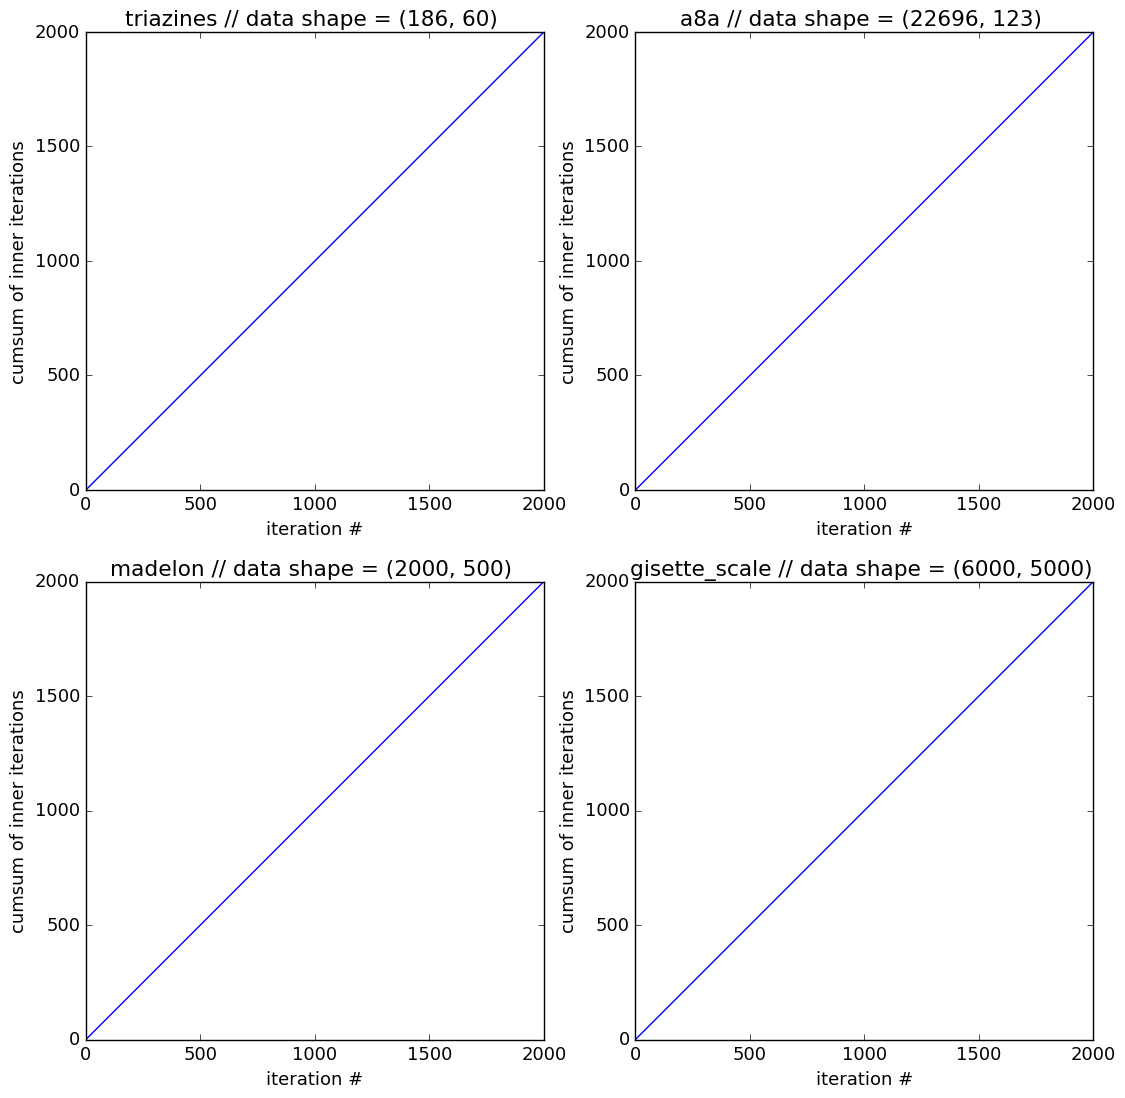
\includegraphics[width=\picwidth]{prox_grad_cumsum.png}\end{center}

    Из графика видно, что для любых данных разных размеров суммарное число итераций одномерного поиска линейное. Т.е. в каждой итерации проксимального метода выполняется всего одна итерация
    одномерного поиска. Таким образом график доказывает, что внутренняя итерация в среднем выполняется не более 2 раз.

    Далее рассмотрим графики зазоров для трех методов при максимальном количестве итераций равным 2000 и точности, раному $10^{-5}$.

    Расположим графики в порядке увеличения количества признаков.
    \def \picwidth {17.5cm}
    \begin{center}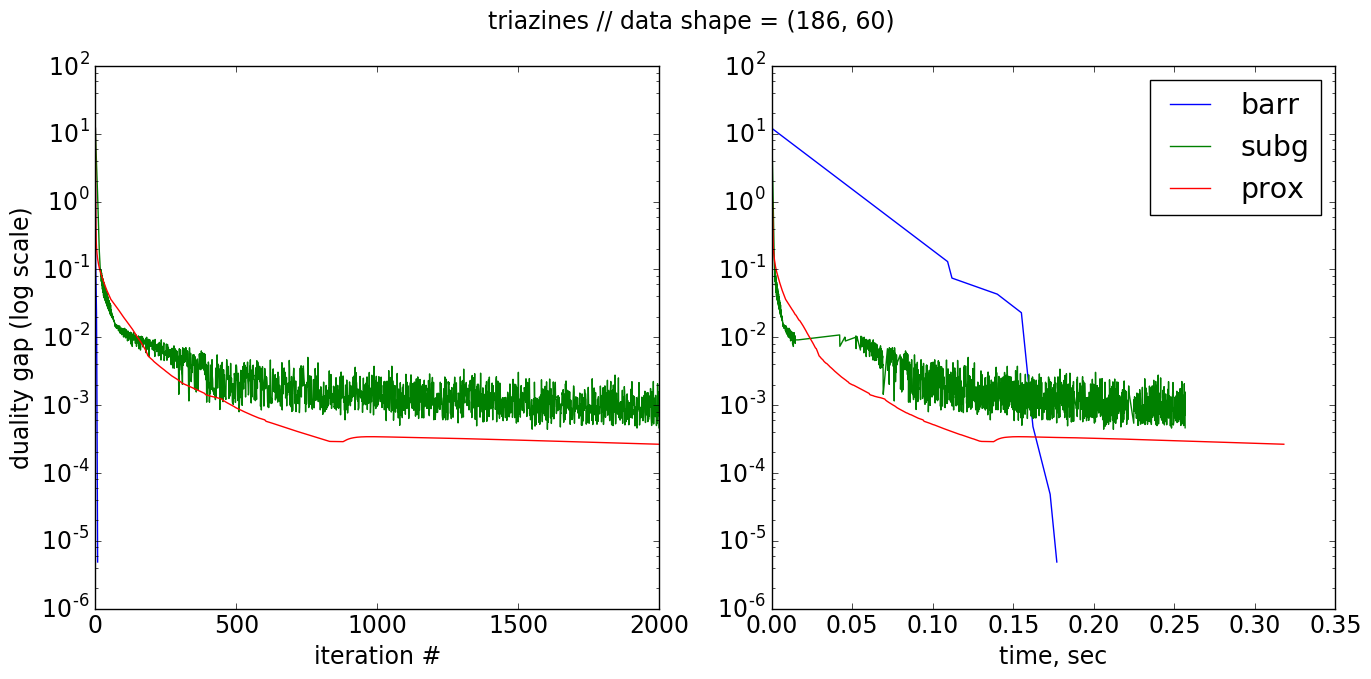
\includegraphics[width=\picwidth]{triazines.png}\end{center}

    Из графика видно, что проксимальный метод сходится до определенного значения зазора -- ассимптоте и далее не оптимизирует функционал. Также и с субградиентным методом.
    Зазор в субградиентном методе в целом уменьшается, но т.к.субградиентный метод строит не обязательно релаксационную последовательность, мы видим колебания.
    Метод барьеров сошелся очень быстро по итерациям и до точности $10^{-2}$ и до точности $10^{-5}$. Но по времени быстрее до $10^{-2}$ сошелся метод субградиентов, а до $10^{-5}$
    сошлелся только метод барьеров.

    % \def \picwidth {17cm}
    Следующая выборка интересна тем, что метод субградиентного спуска и проксимальный метод не показали хорошую точность. И соответственно быстрее всех до точности $10^{-2}$ и $10^{-5}$
    сошелся метод барьеров и по времени и по итерациям.

    \begin{center}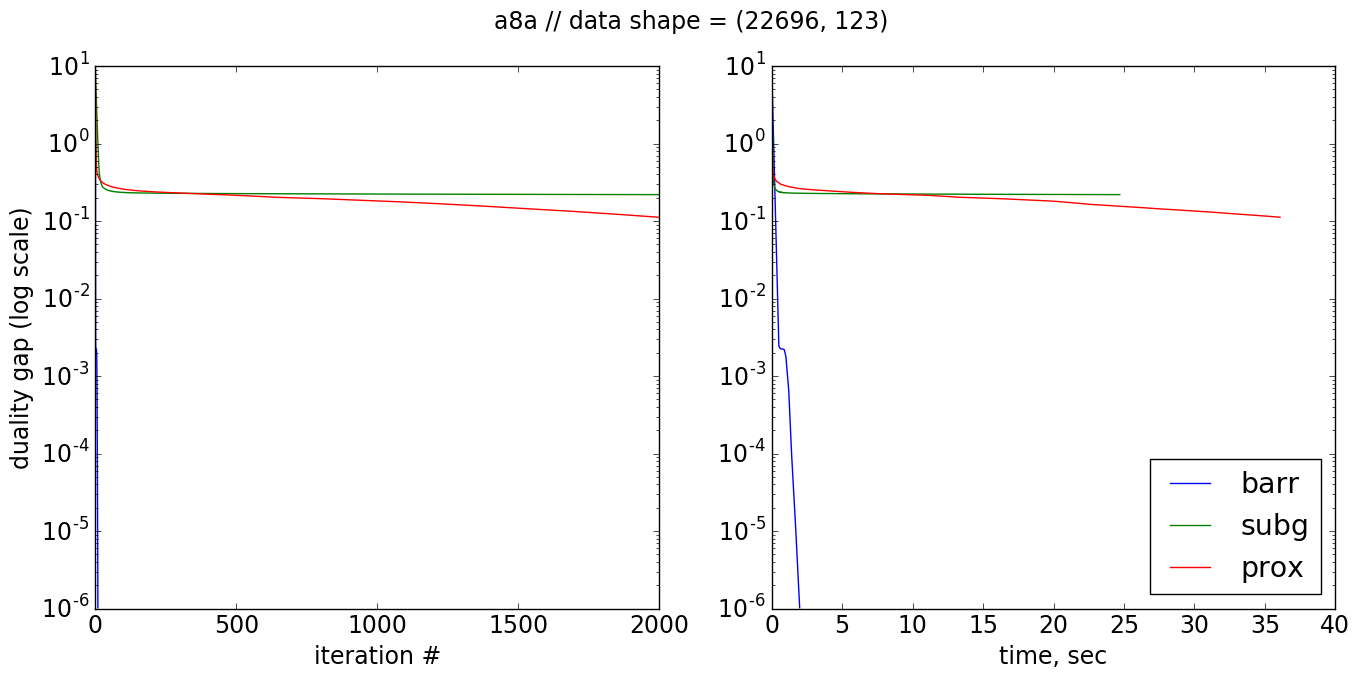
\includegraphics[width=\picwidth]{a8a.png}\end{center}

    % \def \picwidth {17cm}
    Следующий случай примерно аналогичен предыдущему.
    \begin{center}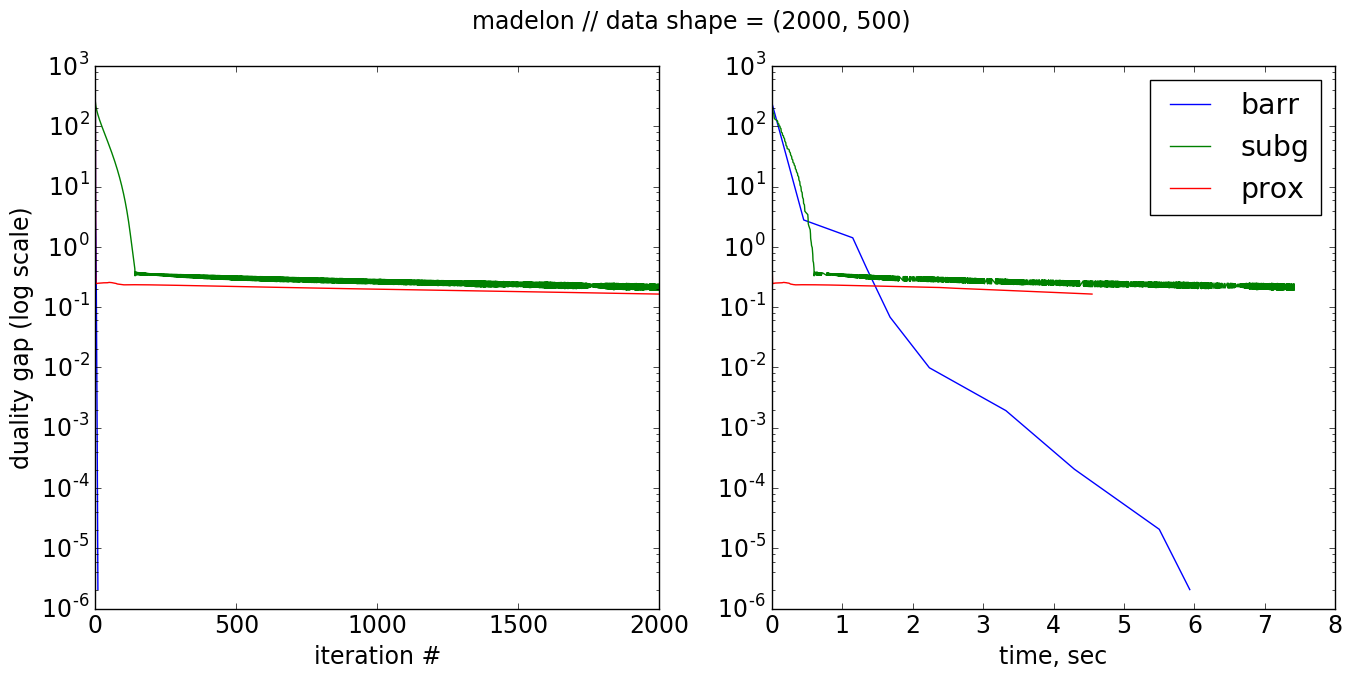
\includegraphics[width=\picwidth]{madelon.png}\end{center}

    % \def \picwidth {17cm}
    Но для данных с большим количеством признаков методы показывают чуть другие результаты. Субградиентный метод падает до ассимптоты медленнее.
    Но проксимальный метод уменьшает зазор также очень быстро до ассимптоты. Метод барьеров также очень быстро сходится по итерациям, но очень долго по времени.
    \begin{center}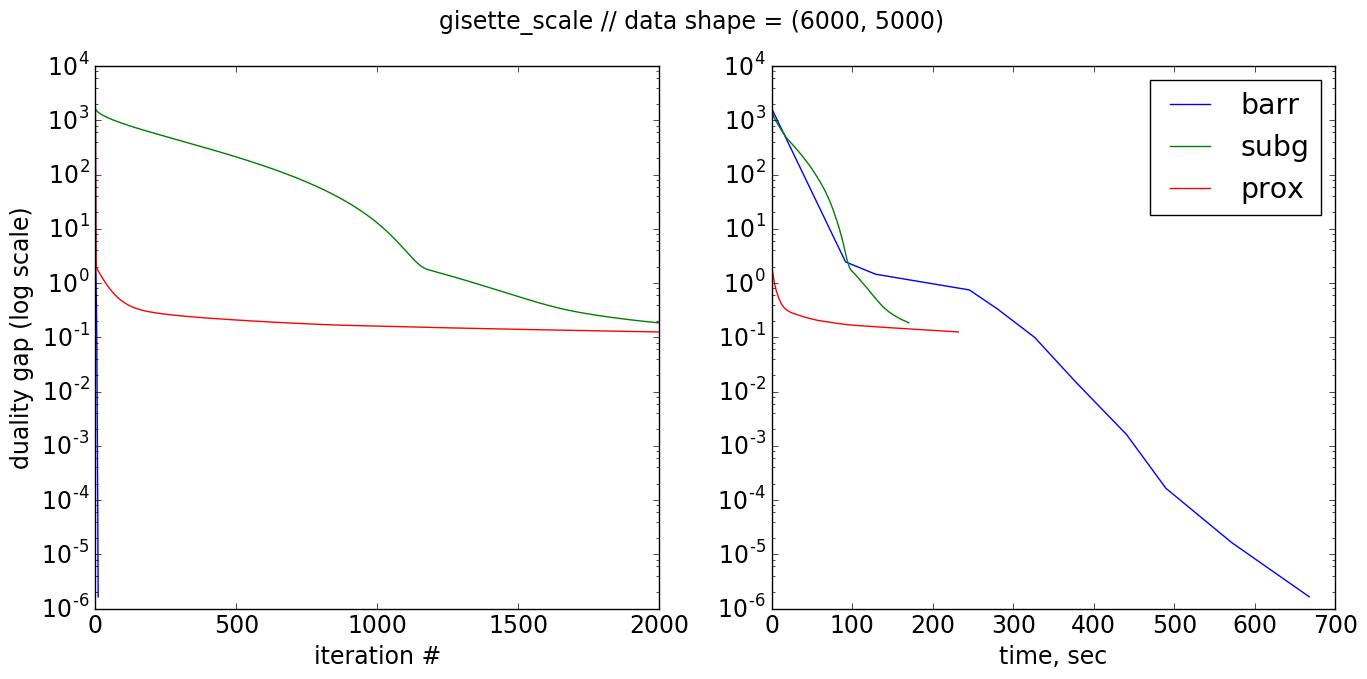
\includegraphics[width=\picwidth]{gisette_scale.png}\end{center}


    \section{Заключение}
    В работе были выведены вспомогательная функция и ньютоновское направление для метода барьеров, исследованы проксимального метод, субградиентный метод и метод барьеров.
    В итоге работы мы получили следующие результаты:
    \begin{enumerate}
        \item Метод барьеров очень быстр по итерация, но не по времени. Чем больше признаков, тем больше время работы.
        \item Проксимальный и субградиентный методы имеют очень маленькую точность, равную $10^{-1}$ в общем случае.
        \item Если нужна большая точность, то лучше использовать метод барьеров, т.к. он достигает хороших точностей.
        \item Если большая точность не нужна, то лучше использовать проксимальный метод, т.к. он сходится меньше чем за секунду до своей ассимптоты
        \item Субградиентный оказался не нужным на фоне других методов. Этот метод не имеет ни быструю сходимость при маленьких точностях, ни большую точность.
    \end{enumerate}

\end{document}
